\documentclass[11pt]{article}
\usepackage[margin=0.9in,top=0.85in,bottom=0.85in]{geometry}
\usepackage{amsmath}
\usepackage{booktabs}
\usepackage{graphicx}
\usepackage[authoryear,round]{natbib}
\usepackage[hidelinks]{hyperref}
\linespread{1.02}
\graphicspath{{../results/}}

\title{Fewer Young Workers in AI-Exposed Occupations:\\ Evidence from Public Survey Microdata}
\author{Moris Wu\thanks{Every number regenerates from one public notebook: \url{https://github.com/mao-data/ai-young-workers}. Public, de-identified data only; no funding; no conflicts of interest. I wrote the code with Claude Code (Anthropic), an AI coding assistant, and checked each result against the notebook output.}}
\date{October 2026}

\begin{document}
\maketitle

\begin{abstract}
\noindent Payroll data suggest that employers are hiring fewer young workers into the occupations most exposed to generative AI, but national surveys have given weaker and less precise evidence. Pooling across all 525 occupations, I find the pattern clearly in public data. In 79 months of Current Population Survey microdata, validated against published employment totals in every month, a one-standard-deviation increase in exposure to large language models is associated with a 0.29 percentage-point fall in the 22--25 share of occupation employment after ChatGPT's release, about 3.8\% of the pre-period mean. There is no such movement before November 2022. The result replicates in the American Community Survey at about half the size and under a usage-based exposure measure. Unemployment rose about equally for young and older workers, which fits reduced hiring of newcomers better than displacement. The estimates are descriptive.
\end{abstract}

\section{Introduction}

Writing code with an AI assistant is fast. Friends of mine who use these tools say they now produce five times as much as before. Whether five times the output is five times the value is less clear. Much of what the tools generate is too voluminous to check line by line, and firms adopting AI want reliability more than volume. When AI narrows the gap between novices and experts, it could make junior workers more useful, since they can now do what used to take years to learn. \citet{althoff2026} argue that, by lowering the skill requirements of tasks, AI lets less-skilled workers compete for jobs that were previously out of reach. But it could also make junior workers less necessary, if the scarce skill becomes judging AI output rather than producing it. Which of these forces dominates should show up first in who gets hired: in the age structure of exposed occupations, well before aggregate unemployment.

Two recent studies look for that trace. \citet{brynjolfsson2026} use payroll records from ADP, a large payroll processor, covering millions of workers and find that employment of 22--25 year-olds in the most AI-exposed occupations stood 19\% below the path of their less-exposed peers by mid-2026, with the gap driven by reduced hiring rather than separations. \citet{massenkoff2026} use the CPS and find that job-finding rates of young workers into highly exposed occupations fell by about 14\% relative to 2022, an estimate they describe as barely significant, with no change in unemployment. Brynjolfsson et al.\ report that the CPS is too noisy in fine age-by-occupation cells, and that in the 2024 ACS the gap between the most and least exposed quintiles is $-0.022$, with a confidence interval that includes zero.

This paper asks whether the payroll pattern is a feature of the ADP sample or is also present in nationally representative data. Instead of comparing a handful of age-by-quintile cells, I estimate an occupation-level regression of the young-worker share on exposure, using all 525 Census occupations with occupation and quarter fixed effects.

The pattern is there. In the CPS, the young share of employment fell more in more-exposed occupations after ChatGPT's release, with flat pre-trends and a null placebo. The same design applied to the ACS gives a smaller but statistically clear decline, and both surveys show it under a second, usage-based exposure measure. The ACS estimate is about half the CPS one, consistent with Brynjolfsson et al.'s finding that survey benchmarks show weaker patterns than ADP. Unlike payroll records, these data are open to anyone, and every estimate here regenerates from a single public notebook, so other researchers can reproduce, check, and extend the results as new months of data arrive.

\section{Data}

\paragraph{CPS microdata.} I use the Census Bureau's basic monthly CPS public-use files from January 2020 to August 2026. The window starts in January 2020 because that is when the CPS adopted 2018 Census occupation codes, so the whole sample uses one occupation classification and no cross-vintage crosswalk is needed. October 2025 is missing: the household survey was not conducted during the federal government shutdown, and the Bureau of Labor Statistics (BLS) publishes no estimate for that month. That leaves 79 monthly files.

I parse the fixed-width files after checking every field position against each year's record layout. Restricting 10.0 million raw records to employed civilian adults leaves 3.7 million person-months, about 3,200 of them employed 22--25 year-olds in a typical month. As a check on the parsing and weights, I sum composite weights over employed respondents in each month and compare the result with the published BLS employment level (series LNU02000000). The two agree in all 79 months, with a maximum deviation of 0.0003\%.

\paragraph{Exposure.} The main measure is the occupation-level exposure score of \citet{eloundou2024}, the share of an occupation's tasks that a large language model could perform substantially faster (their $\beta$ measure, as rated by OpenAI's GPT-4 model). Scores are defined for occupations in the Occupational Information Network (O*NET), so I map them to 2018 Standard Occupational Classification (SOC) codes and then to Census occupation codes. Where a Census code combines several SOC occupations, I average over its members, falling back to the parent group for residual ``all other'' codes that have no O*NET profile. This matches 525 of 526 Census occupations; the exception is the armed forces, outside the civilian sample. As a second measure I use the observed exposure of \citet{massenkoff2026}, which weights tasks by how often they appear in actual automated use of Claude. The two measures are correlated at 0.67 (employment-weighted).

\paragraph{ACS.} To check the CPS results against an independent survey, I use the American Community Survey 1-year files for 2021--2024. The ACS uses the same occupation codes, so the exposure mapping carries over unchanged, and it has about 105,000 employed 22--25 year-olds per year, some thirty times a CPS month. Its employment totals run 2.5--3.8\% above the CPS, as expected from its broader coverage.

\section{Empirical approach}

For occupation $o$ in quarter $t$, let $Y_{ot}$ be the share of the occupation's employment aged 22--25, in percentage points. Quarterly values average the monthly weighted counts that are available, so the missing October 2025 does not distort the fourth quarter of that year. I estimate
\begin{equation}
Y_{ot} = \alpha_o + \lambda_t + \sum_{k \neq \text{2022Q3}} \beta_k \, E_o \, \mathbf{1}[t = k] + \varepsilon_{ot},
\label{eq:es}
\end{equation}
where $E_o$ is standardized exposure and $\alpha_o$ and $\lambda_t$ are occupation and quarter fixed effects. The sample runs from 2021Q1, after the pandemic collapse, to 2026Q3. Observations are weighted by 2022 occupation employment and standard errors are clustered by occupation. The omitted quarter, 2022Q3, is the last full quarter before ChatGPT's release on 30 November 2022. Each $\beta_k$ measures whether the young share moved differently in more-exposed occupations in quarter $k$; coefficients near zero before 2022Q4 support the parallel-trends assumption. A pooled version replaces the quarter-specific terms with a single interaction $E_o \times \text{Post}_t$.

Because the outcome is a share, it nets out shocks that hit an occupation as a whole, such as the 2023 slowdown in technology hiring, as long as they affect all ages alike.

\section{Results}

Figure~\ref{fig:index} shows the raw pattern. Employment of 22--25 year-olds in the least exposed quintile grew by about 14\% between 2022Q3 and 2026Q3, while in the most exposed quintile it ended below its 2022Q3 level. Among 35--49 year-olds the ordering is reversed, and the most exposed quintile grew fastest. The young series do not fall smoothly. In the most exposed quintile, young employment rose in early 2023, swung between about 96 and 107 through 2025, and dropped to about 93 in 2026. Some of this movement is sampling noise, since each quintile holds only about 600 employed 22--25 year-olds in a given month, which is why the regressions below pool across occupations rather than read the lines.

\begin{figure}[!htbp]
\centering
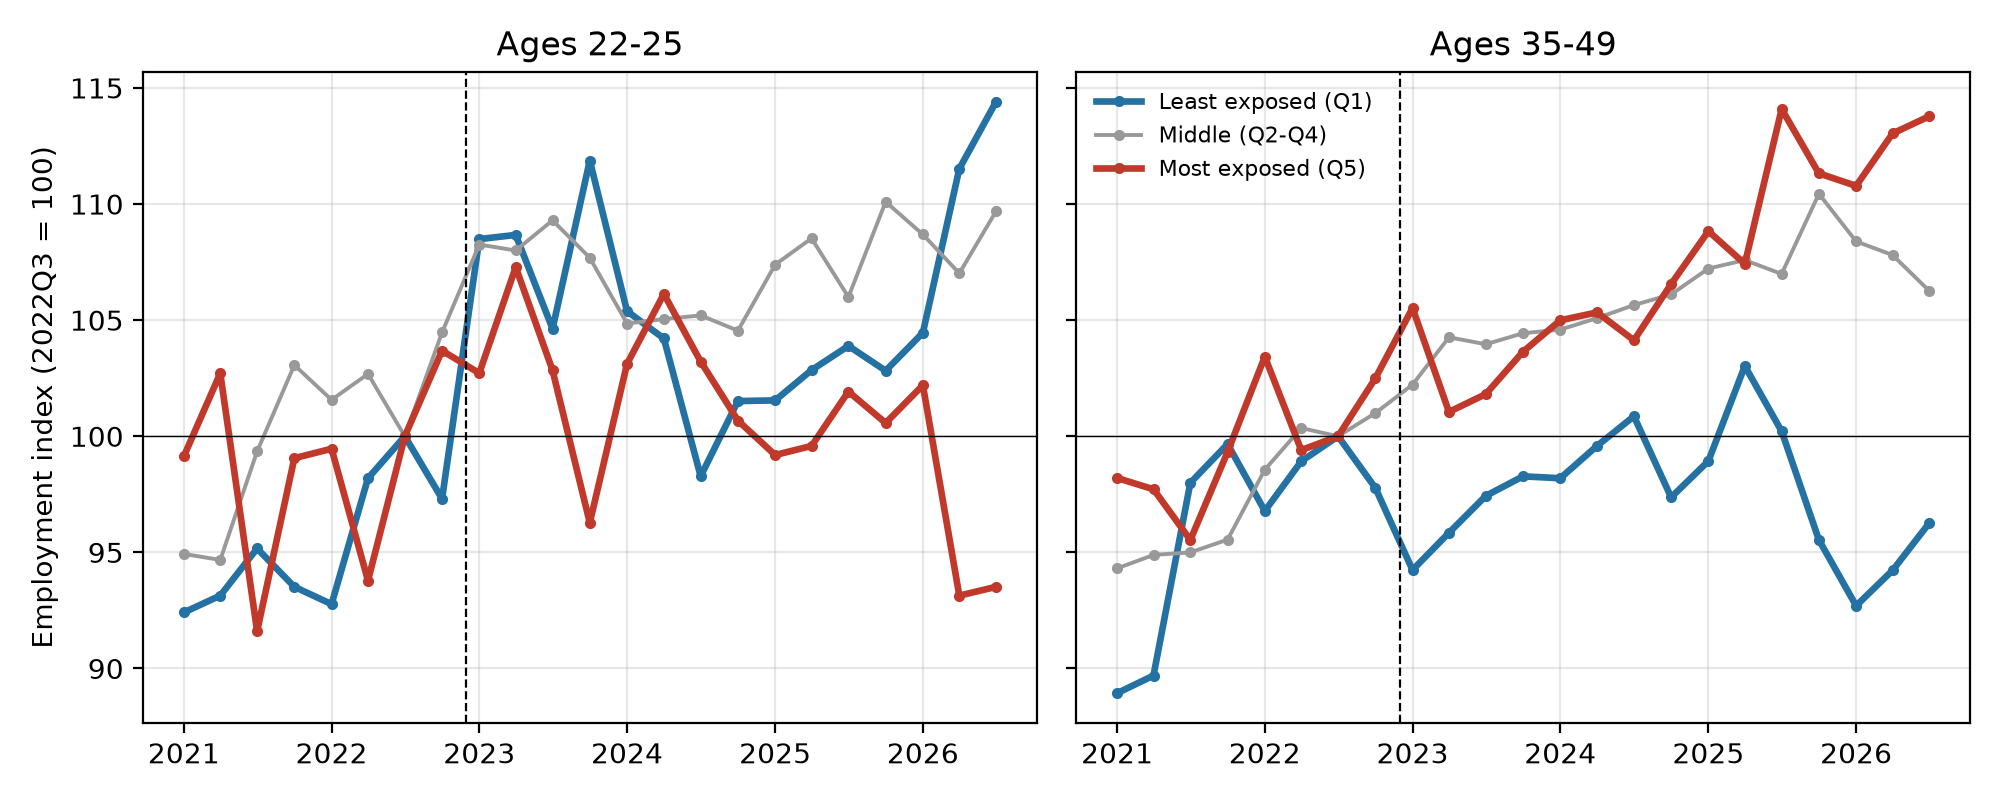
\includegraphics[width=0.82\textwidth]{fig1_index_by_quintile.png}
\caption{Employment by exposure quintile, indexed to 2022Q3 = 100. Quintiles are weighted so that each holds about one-fifth of 2022 employment. The dashed line marks ChatGPT's release. Source: CPS basic monthly files.}
\label{fig:index}
\end{figure}

Figure~\ref{fig:es} plots the event-study coefficients from equation~\eqref{eq:es}. Before ChatGPT they are small and scattered around zero. From 2023 onward they are negative in every quarter, close to zero in mid-2024, and largest in 2026. Pooling the post period, a one-standard-deviation increase in exposure is associated with a 0.29 percentage-point lower young share (Table~\ref{tab:main}, row 1). Against a 2022Q3 mean of 7.74\%, that is a relative decline of about 3.8\%. Because the outcome is a share rather than a headcount, this number is not directly comparable to the 19\% gap in ADP.

\begin{figure}[!htbp]
\centering
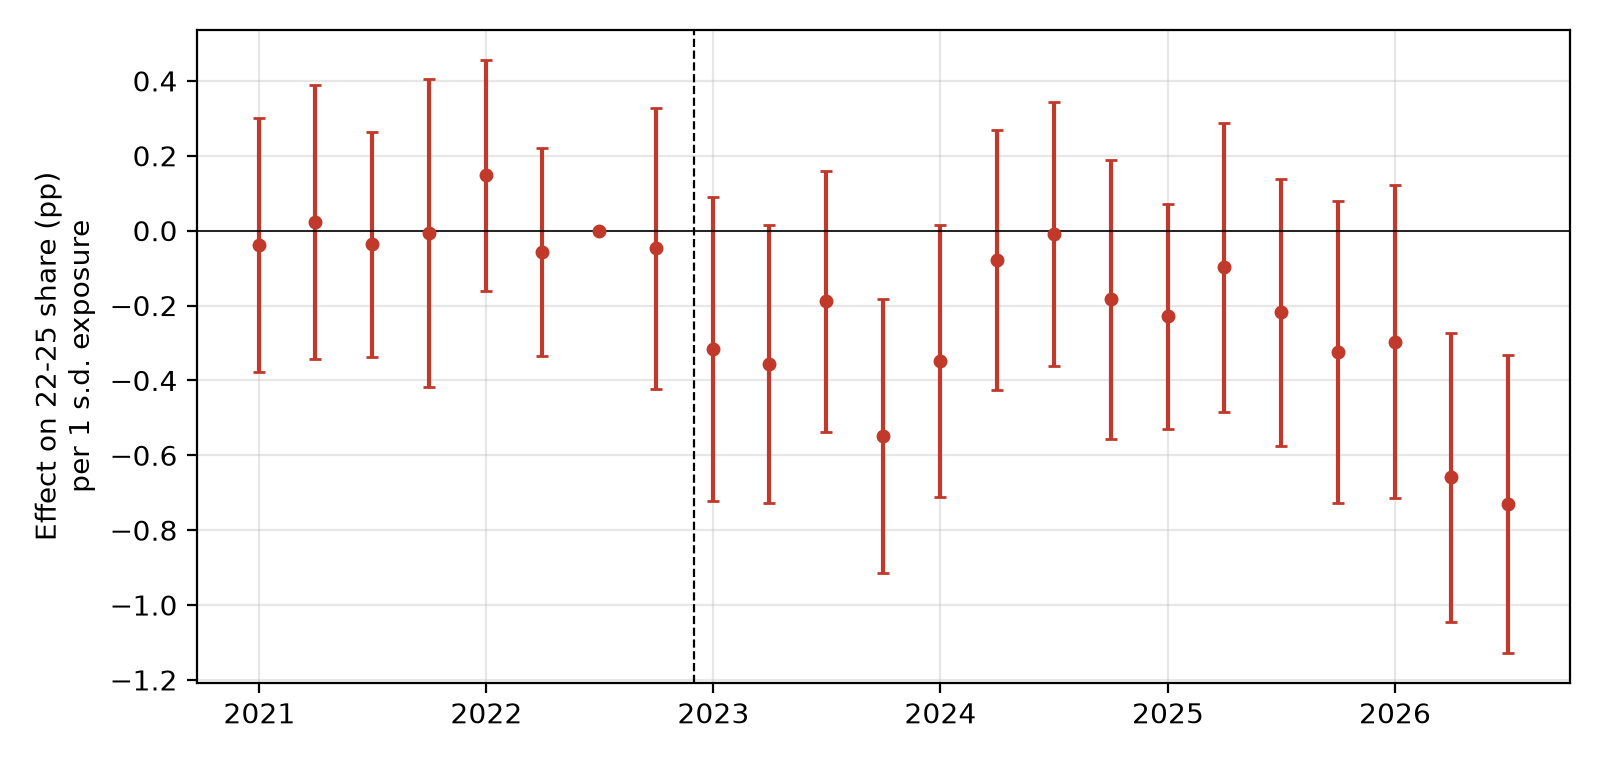
\includegraphics[width=0.58\textwidth]{fig2_event_study.png}
\caption{Event-study estimates of $\beta_k$ from equation~\eqref{eq:es}, with 95\% confidence intervals. The omitted quarter is 2022Q3; the dashed line marks ChatGPT's release.}
\label{fig:es}
\end{figure}

Table~\ref{tab:main} reports alternative specifications. The estimate barely moves with human-rated exposure, when the sample is restricted to wage and salary workers (the population covered by payroll data), or when computer and mathematical occupations are dropped. The last check matters because these occupations are among the most exposed and were also hit by the 2023 tech layoffs, which coincided with rising interest rates. Ending the sample in 2025Q4 lowers the estimate to $-0.23$, still significant, so the result does not rest on 2026 alone. A placebo that moves the event to 2021Q4 and uses only pre-ChatGPT data gives $+0.04$ (s.e.\ 0.12).

\begin{table}[!htbp]
\centering
\footnotesize
\caption{Effect of exposure on the 22--25 share of occupation employment after ChatGPT}
\label{tab:main}
\begin{tabular}{lrrr}
\toprule
 & Coefficient & s.e. & $p$ \\
\midrule
\multicolumn{4}{l}{\textit{A. CPS, quarterly, 2021Q1--2026Q3}} \\
(1) Baseline: GPT-4 exposure & $-0.294$ & 0.089 & 0.001 \\
(2) Human-rated exposure & $-0.290$ & 0.090 & 0.001 \\
(3) Wage and salary workers only & $-0.308$ & 0.096 & 0.001 \\
(4) Excluding computer \& math occupations & $-0.308$ & 0.092 & 0.001 \\
(5) Sample ends 2025Q4 & $-0.231$ & 0.089 & 0.009 \\
(6) Ages 22--29 & $-0.415$ & 0.119 & 0.001 \\
(7) Observed exposure \citep{massenkoff2026} & $-0.183$ & 0.070 & 0.009 \\
(8) Placebo: event in 2021Q4, pre-ChatGPT data only & $+0.044$ & 0.124 & 0.721 \\
\midrule
\multicolumn{4}{l}{\textit{B. Annual, 2021--2024 (post = 2023--2024)}} \\
(9) CPS, GPT-4 exposure & $-0.276$ & 0.105 & 0.008 \\
(10) ACS, GPT-4 exposure & $-0.149$ & 0.056 & 0.007 \\
(11) ACS, human-rated exposure & $-0.164$ & 0.063 & 0.009 \\
(12) ACS, excluding computer \& math occupations & $-0.137$ & 0.058 & 0.018 \\
(13) ACS, observed exposure & $-0.122$ & 0.049 & 0.013 \\
(14) ACS, ages 22--29 & $-0.060$ & 0.076 & 0.430 \\
\bottomrule
\end{tabular}
\par\vspace{4pt}
\begin{minipage}{0.92\textwidth}
\footnotesize \textit{Notes:} Coefficient on standardized exposure $\times$ post-ChatGPT, in percentage points of the young share. Occupation and period fixed effects; weights are 2022 occupation employment; standard errors clustered by occupation (525 occupations; 510 for observed exposure).
\end{minipage}
\end{table}

Without employment weights the CPS coefficient falls to $-0.09$ and is not significant, but this reflects noise: the median occupation has only about 124 young-worker observations in the whole sample. Among the 152 occupations with at least 300, the unweighted estimate is $-0.46$ ($p = 0.007$). Dropping any one of the 30 largest occupations leaves the coefficient between $-0.31$ and $-0.28$, and none of 1,000 random reassignments of exposure across occupations produces one as large.

Panel B turns to the ACS. Applying the same design to annual data for 2021--2024 gives $-0.15$ ($p = 0.007$), about half the CPS estimate over the same years ($-0.28$). By year, the ACS coefficient is close to zero in 2021 and 2023 and $-0.21$ in 2024 ($p = 0.006$), so in this survey the decline appears late. Timing explains part of the gap with the full CPS estimate, since the ACS ends in 2024, before the largest CPS coefficients in 2026. It does not explain all of it: over the same 2021--2024 window the CPS estimate is still about twice the ACS one. The smaller CPS cells are noisier, and the larger ACS may be closer to the true size, in line with the attenuation in survey benchmarks that \citet{brynjolfsson2026} report. In the ACS the effect is confined to ages 22--25 and disappears for 22--29 (row 14), which suggests that conditions change fastest for the newest entrants; in the CPS it is larger for the wider band.

\section{Entry or displacement?}

A falling young share could mean that firms dismiss young workers or that they hire fewer of them. The CPS can separate these because it records the last occupation of unemployed respondents, which payroll data do not. If AI displaced young incumbents, their unemployment rate should rise more than older workers' in exposed occupations. It does not. Using the same design with unemployment as the outcome, a one-standard-deviation increase in exposure is associated with a 0.58 percentage-point higher unemployment rate for 22--25 year-olds (s.e.\ 0.21) and a 0.55 point higher rate for 35--49 year-olds (s.e.\ 0.11). Unlike \citet{massenkoff2026}, who find no change in unemployment in exposed occupations, I find a rise, but it is nearly identical for the two age groups. A young-specific fall in employment share without a young-specific rise in unemployment fits reduced entry better than displacement. The cheapest ways for a firm to adjust, leaving departures unfilled, freezing junior hiring, and cutting costs, all work at the entry margin, and none of them raises unemployment among young incumbents. This agrees with the hiring channel that \citet{brynjolfsson2026} document in payroll data and with the decline in job-finding rates in \citet{massenkoff2026}. I compare the two point estimates rather than testing their difference formally.

\section{Limitations and conclusion}

These estimates are descriptive: exposure is not randomly assigned, and exposed occupations may differ in other ways that matter for young workers after 2022. The most obvious alternative, the tech-sector slowdown, does not explain the result, but others remain. \citet{brynjolfsson2026} find that their pattern weakens when they control for occupational education levels; I do not test this here, and it may represent either a confound or the channel through which AI operates. The ACS currently ends in 2024; the 2025 file will show whether the larger CPS coefficients for 2026 reflect a strengthening trend or sampling noise.

Within those limits, public surveys show the same pattern as private payroll data: in two independent surveys and under two exposure measures, fewer young people are entering exposed occupations, without more of them losing jobs there. One reading, which these data cannot test directly, is that when AI can do much of the routine work, firms put their resources into workers who know the job well enough to judge what the tool produces, and less into newcomers who can operate the tool but cannot yet tell good output from bad. Three extensions would sharpen this: comparing small and large firms, finding which industries respond most, and asking whether demand rises steadily with experience or differs between workers with ten, twenty, and thirty years in the job. For now, the evidence points to fewer openings and fewer jobs for young workers in exposed occupations, and plausibly to more being asked of those who get in.

\begin{thebibliography}{9}

\bibitem[Althoff and Reichardt(2026)]{althoff2026}
Althoff, Lukas, and Hugo Reichardt. 2026.
``Task-Specific Technical Change and Comparative Advantage.''
NBER Working Paper 35353.

\bibitem[Brynjolfsson, Chandar, and Chen(2026)]{brynjolfsson2026}
Brynjolfsson, Erik, Bharat Chandar, and Ruyu Chen. 2026.
``Canaries in the Coal Mine? Six Facts about the Recent Employment Effects of Artificial Intelligence.''
Working paper, Stanford Digital Economy Lab, August 2026 version.

\bibitem[Eloundou et~al.(2024)]{eloundou2024}
Eloundou, Tyna, Sam Manning, Pamela Mishkin, and Daniel Rock. 2024.
``GPTs Are GPTs: Labor Market Impact Potential of LLMs.''
\textit{Science} 384 (6702): 1306--1308. \url{https://doi.org/10.1126/science.adj0998}.

\bibitem[Massenkoff and McCrory(2026)]{massenkoff2026}
Massenkoff, Maxim, and Peter McCrory. 2026.
``Labor Market Impacts of AI: A New Measure and Early Evidence.''
Report, Anthropic, March 5, 2026. Data: Anthropic Economic Index, \texttt{labor\_market\_impacts/job\_exposure.csv}.

\bibitem[U.S. Census Bureau(2026)]{census}
U.S. Census Bureau. 2020--2026. Current Population Survey basic monthly public-use files; American Community Survey 1-year Public Use Microdata Sample, 2021--2024.

\end{thebibliography}

\end{document}
